\begin{frame}{Introduction}

	\begin{minipage}[c][.23\textheight]{.8\textwidth}
		\begin{itemize}
			\itemfill
			\item in early 90s all SM particles except H and t-quark discovered
			\item beauty discovery \ra weak isospin partner was undoubted
			\item quark masses are fundamental parameters in the SM
		\end{itemize}
	\end{minipage}
	\begin{minipage}{.18\textwidth}
		\fig{B1}{.2}
	\end{minipage}
	
	\begin{itemize}\itemfill
		\item early estimates: $\z{m}_{\z{t}} \approx 3 \z{m}_{\z{b}} \approx \SI{15}{\giga\electronvolt}$
		\item many new accelerator could only push limits higher:
		\item TRISTAN ($e^+e^-$) at KEK (Tsukuba, Japan) with $\sqrt{s} = \SI{61.4}{\giga\electronvolt}$ \ra \SI{30.2}{\giga\electronvolt}
		\item Sp$\overline{\z{p}}$S at CERN with $\sqrt{s} = \SI{630}{\giga\electronvolt}$ \ra \SI{69}{\giga\electronvolt}
		\item SLC ($e^+e^-$) at Stanford and LEP ($e^+e^-$) at CERN \ra $\sfrac{1}{2} \z{m}_{\z{t}}$
		\item hadron collider needed (\ra Tevatron)
	\end{itemize}
	
\end{frame}
%%%%%%%%%%%%%%%%%%%%%%%% FRAME 1 %%%%%%%%%%%%%%%%%%%%%%%%%%%%%%%
\begin{frame}{Decay Channels (1)}

	\begin{itemize}\itemfill
		\item estimate on $\z{m}_{\z{t}}$ in 1994: \SI{\sim180}{\giga\electronvolt}
		\item prior to discovery: behaviour completely predicted by SM
		\item $\z{m}_{\z{t}} > \z{m}_{\z{W}}$ \ra main decay channel (\SI{\sim95}{\%}):\ka{\usebeamercolor[fg]{title}\textbf{t\ch{->}$\z{W}^+\z{b}$}}
		\begin{equation*} \Upgamma_{\z{t}} = \frac{\z{G}_{\z{F}}\z{m}_{\z{t}}^{3}}{8\uppi\sqrt{2}}\left(1 - \frac{\z{m}_{\z{W}}^{2}}{\z{m}_{\z{t}}^{2}}\right)^{2}\left(1 + 2\frac{\z{m}_{\z{W}}^{2}}{\z{m}_{\z{t}}^{2}}\right)\end{equation*}
		\item width for the expected mass: \SI{\sim1}{\giga\electronvolt} \ra decay before hadronisation
	\end{itemize}
	
	\begin{figure}\vspace*{-10pt}
		\centering
		\subfig[.3]{tWbq}{.25}{\SI{\sim60}{\%}}
		\subfig[.3]{tWbl}{.25}{\SI{\sim40}{\%}}
	\end{figure}\vspace*{-10pt}
	
	\begin{itemize}\itemfill
		\item leptonic decay equally splits up into $e$, $\upmu$ and $\uptau$
	\end{itemize}

\end{frame}
%%%%%%%%%%%%%%%%%%%%%%%% FRAME 2 %%%%%%%%%%%%%%%%%%%%%%%%%%%%%%%
\begin{frame}{Decay Channels (2)}

	\begin{itemize}\itemfill
		\item top mostly pair produced via $\z{q}\overline{\z{q}}$\ch{->}$\z{t}\overline{\z{t}}$ or gluon fusion: $\z{g}\z{g}$\ch{->}$\z{t}\overline{\z{t}}$  
		\item main decay of the top pair: $\z{t}\overline{\z{t}}$\ch{->}$\z{W}^+\z{b}\z{W}^-\overline{\z{b}}$
		\item b decay:
	\end{itemize}
	
	\begin{figure}\vspace*{-10pt}
		\centering
		\subfiga[.3]{BDec2}{.25}\hspace*{10pt}
		\subfiga[.4]{BDec1}{.25}
	\end{figure}
	
	\begin{itemize}\itemfill
		\item typical signals:
		\begin{itemize}
			\item 2 b-jets + dilepton ($e^+e^-$, $\upmu^+\upmu^-$, $e^+\upmu^-$, $\upmu^+e^-$)
			\item 2 b-jets + single lepton + two jets
			\item 2 b-jets + 4 jets
		\end{itemize}
		\item huge background on pure QCD process due to other more common QCD processes
		\item how to discriminate b-jets from other jets?
	\end{itemize}

\end{frame}
%%%%%%%%%%%%%%%%%%%%%%%% FRAME 3 %%%%%%%%%%%%%%%%%%%%%%%%%%%%%%%
\begin{frame}{B-Tagging}

	\begin{itemize}\itemfill
		\item how to discriminate b-jets from other jets?
	\end{itemize}

\end{frame}
%%%%%%%%%%%%%%%%%%%%%%%% FRAME 4 %%%%%%%%%%%%%%%%%%%%%%%%%%%%%%%
\begin{frame}{$\z{t}\overline{\z{t}}$ Cross Section}

	\vspace*{-10pt}\fig{ttcs}{.65}\vspace*{-10pt}
	
	\begin{itemize}\itemfill
		\item cross section extracted from SM
		\item Tevatron Lumi in 1995: \SI{10e30}{\per\centi\meter\squared\per\second}
		\begin{equation*} \z{R}_{\z{t}\overline{\z{t}}} = \upsigma_{\z{t}\overline{\z{t}}}\mathscr{L} = \SI{.1}{\hertz}\end{equation*}

	\end{itemize}

\end{frame}
\subsection{Discovery at CDF}
%%%%%%%%%%%%%%%%%%%%%%%% FRAME 5 %%%%%%%%%%%%%%%%%%%%%%%%%%%%%%%
\begin{frame}{Discovery Paper (1)}
	\fig{TDis1}{.84}
\end{frame}
%%%%%%%%%%%%%%%%%%%%%%%% FRAME 6 %%%%%%%%%%%%%%%%%%%%%%%%%%%%%%%
\begin{frame}{Discovery Paper (2)}
	\fig{TDis2}{.84}
\end{frame}
%%%%%%%%%%%%%%%%%%%%%%%% FRAME 7 %%%%%%%%%%%%%%%%%%%%%%%%%%%%%%%
\begin{frame}{CDF Detector (1)}[plain]
	\begin{tikzpicture}[remember picture,overlay]
		\node[at=(current page.center)] {
			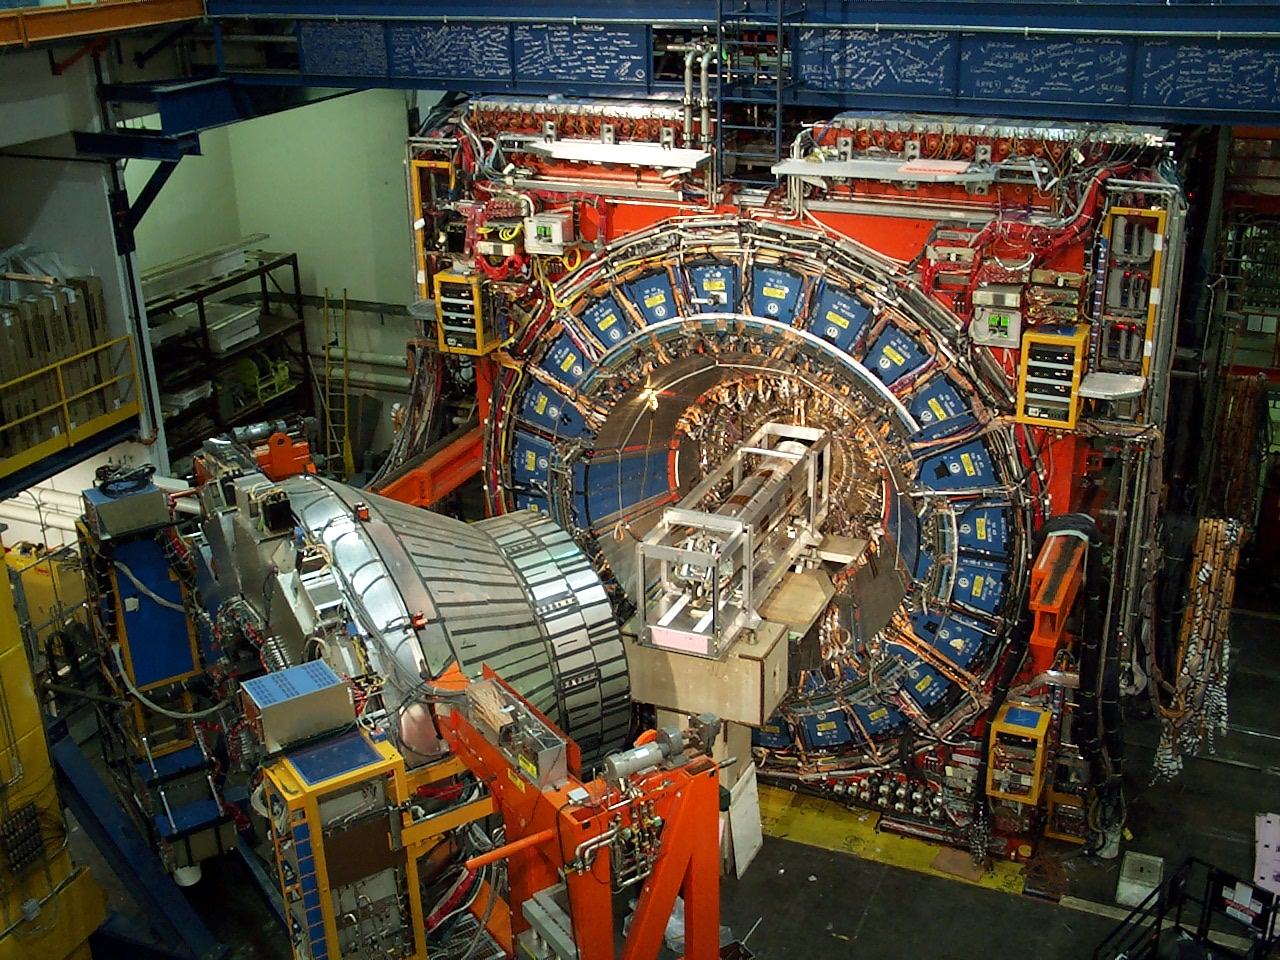
\includegraphics[width=\paperwidth]{cdfdet}
		};
	\end{tikzpicture}
\end{frame}
%%%%%%%%%%%%%%%%%%%%%%%% FRAME 8 %%%%%%%%%%%%%%%%%%%%%%%%%%%%%%%
\begin{frame}{CDF Detector}
	\fig{CDFDet1}{.84}
\end{frame}
%%%%%%%%%%%%%%%%%%%%%%%% FRAME 9 %%%%%%%%%%%%%%%%%%%%%%%%%%%%%%%
\begin{frame}{Introduction}
	
	\begin{itemize}\itemfill
		\item paper from 1994 with estimate on mass and cross section
		\item using dataset of \SI{19}{\per\pico\barn} + \SI{47}{\per\pico\barn} (\ra $\sim$ 400 events)
		\item looking at two decay channels
		\begin{itemize}
			\item dilepton
			\item lepton + jets
		\end{itemize}
		\item both data samples subsets of events with isolated leptons with high $P_{T}>\SI{20}{\giga\electronvolt}$
		\item cut on invariant mass of dilepton $\SI{75}{\giga\electronvolt}<\z{m}_{\z{I}}<\SI{105}{\giga\electronvolt}$ \ra exclude Z events
		\item main background reduction by b-tagging
		\begin{itemize}
			\item reconstruction of secondary vertices from b decay in SVX \ra SVX tag 
			\item finding additional leptons from b decay in ECAL \ra SLT tag 
		\end{itemize}
	\end{itemize}

\end{frame}
%%%%%%%%%%%%%%%%%%%%%%%% FRAME 10 %%%%%%%%%%%%%%%%%%%%%%%%%%%%%%%
\begin{frame}{Lepton + Jets Channel}
	
	\underline{\textbf{SVX tagging:}}\vspace*{5pt}
	\begin{itemize}\itemfill 
		\item search for secondary vertices with three ore more tracks
		\item then search for two ore more tracks with more stringed track and vertex quality
		\item efficiency estimated by $e$, $\upmu$ samples with enriched b decays (\SI{96}{\%} agreement to MC)
		\item tagging efficiency: \SI{42\pm5}{\%}
	\end{itemize}
	
	\begin{minipage}[c][.30\textheight]{.64\textwidth}
	 	\begin{itemize}\itemfill
			\item backgrounds from recoil of heavy quark pairs against W and mistags
	 	 	\item for $\z{W}+\ge3$ jets: observation of \SI{27}{tags} with bg of \SI{6.7\pm2.1}{tags}
	 	 	\item decay lifetime of SVX tags agrees well with MC
	 	\end{itemize}
	\end{minipage}
	\begin{minipage}{.33\textwidth}
		\fig{CDFRes1}{.45}
	\end{minipage}

\end{frame}
%%%%%%%%%%%%%%%%%%%%%%%% FRAME 11 %%%%%%%%%%%%%%%%%%%%%%%%%%%%%%%
\begin{frame}{Dilepton Channel}
	
	\begin{minipage}[c][.30\textheight]{.64\textwidth}
		\begin{itemize}\itemfill 
			\item major backgrounds:
			\begin{itemize}
				\item Drall-Yan process
				\item Z\ch{->}$\uptau\uptau$
				\item misidentified hadrons
				\item WW, b$\overline{\z{b}}$
			\end{itemize}
		\end{itemize}
	\end{minipage}
	\begin{minipage}{.33\textwidth}
		\fig{DrellYan}{.3}
	\end{minipage}

\end{frame}
